% !TeX spellcheck = en_GB

%%%%%%%%%%%%%%%%%%%%%%%%%%%%%%%%%%%%%%%%%%%%%%%%%%%%%%%%%%%%%%%%%%%%%%%%
\chapter{Conclusion}
\label{chap:conclusion}

This chapter finishes the thesis by summarizing its main points. It also includes suggestions how the plug-in could be further improved in the future.

\section{Summary}
\label{sec:summary}

This section gives a high level overview over the main points of this thesis. \\
In Section \ref{sec:implementationDetails}, the implementation is described. The section gave a detailed overview over how the plug-in was designed to meet the goals defined in Section \ref{sec:goals}. Section \ref{sec:encounteredProblems} described previous architectures and which problems they had.\\
The main point of this thesis is the description how the current implementation meets these goals and how the problems which occurred during development were solved.

\subsubsection{Goals}

Three goals which the plug-in should meet were defined.

\begin{enumerate}[label=(\labelenum{G}{{\arabic*}}), wide, labelwidth=!, labelindent=0pt]
\setlength{\parskip}{0pt}
    \item \textbf{Easy-to-understand visualization of the encryption process}\\
    The first goal was met by creating a simple but thought-through user interface for the plug-in visualization.
    
\begin{figure}
\begin{subfigure}{0.85\textwidth}
  \centering
  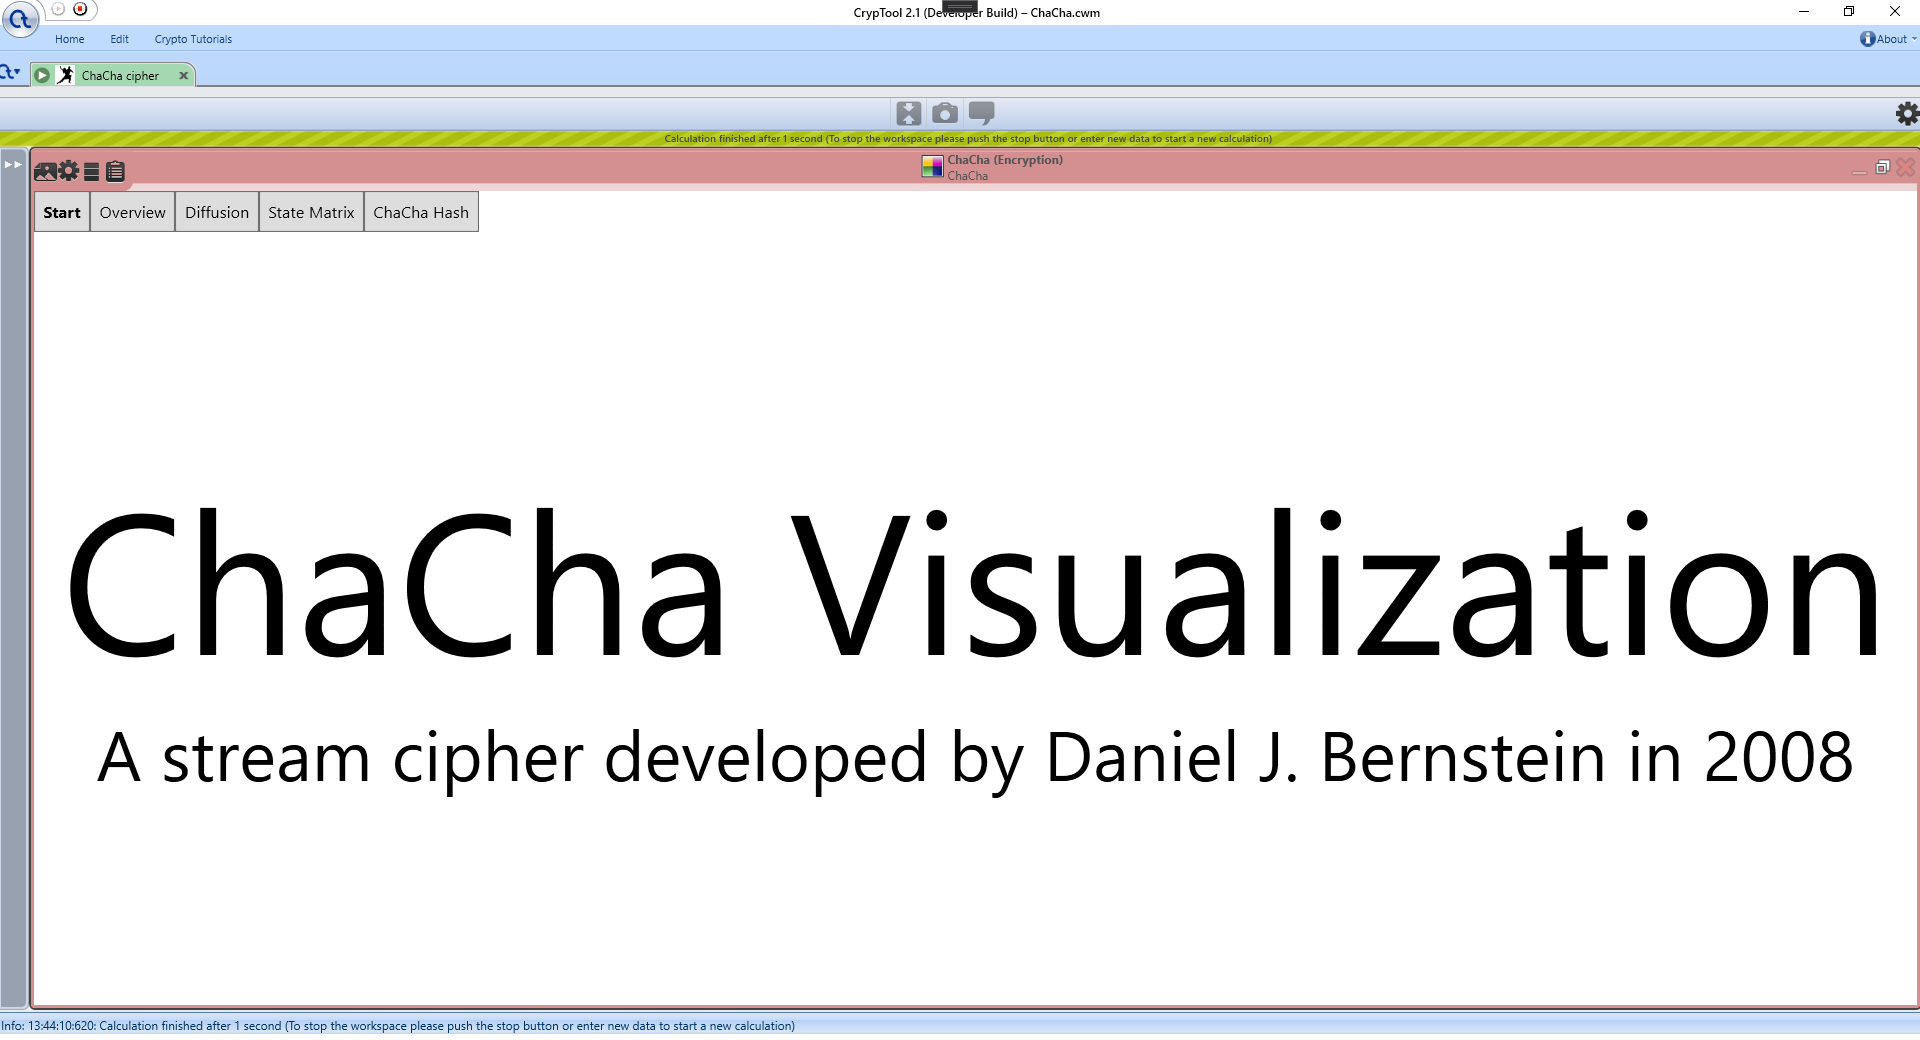
\includegraphics[width=\textwidth]{figures/ct2/all-pages/1-start.png}
  \caption{Landing page}
  \label{fig:all-pages.landing.page}
\end{subfigure}
\begin{subfigure}{0.85\textwidth}
  \centering
  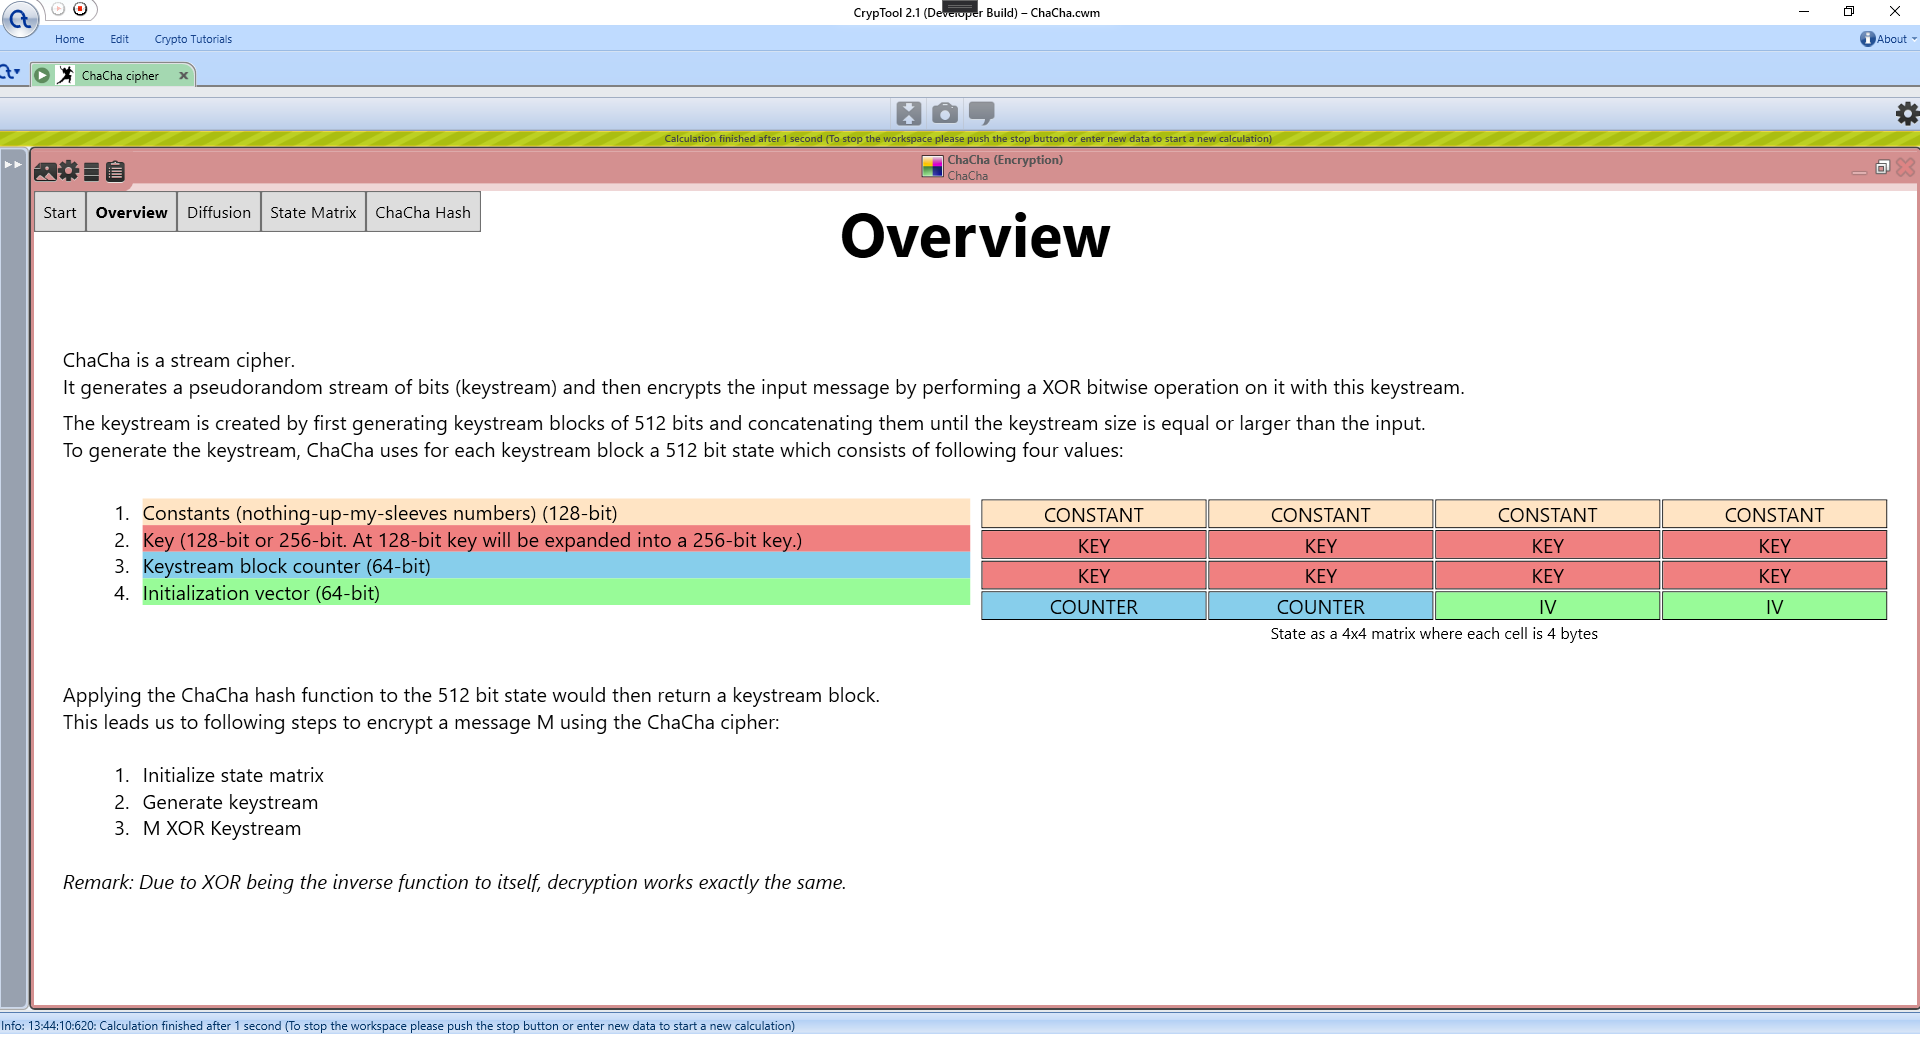
\includegraphics[width=\textwidth]{figures/ct2/all-pages/2-overview.png}
  \caption{Overview page}
  \label{fig:all-pages.overview.page}
\end{subfigure}
\begin{subfigure}{0.85\textwidth}
  \centering
  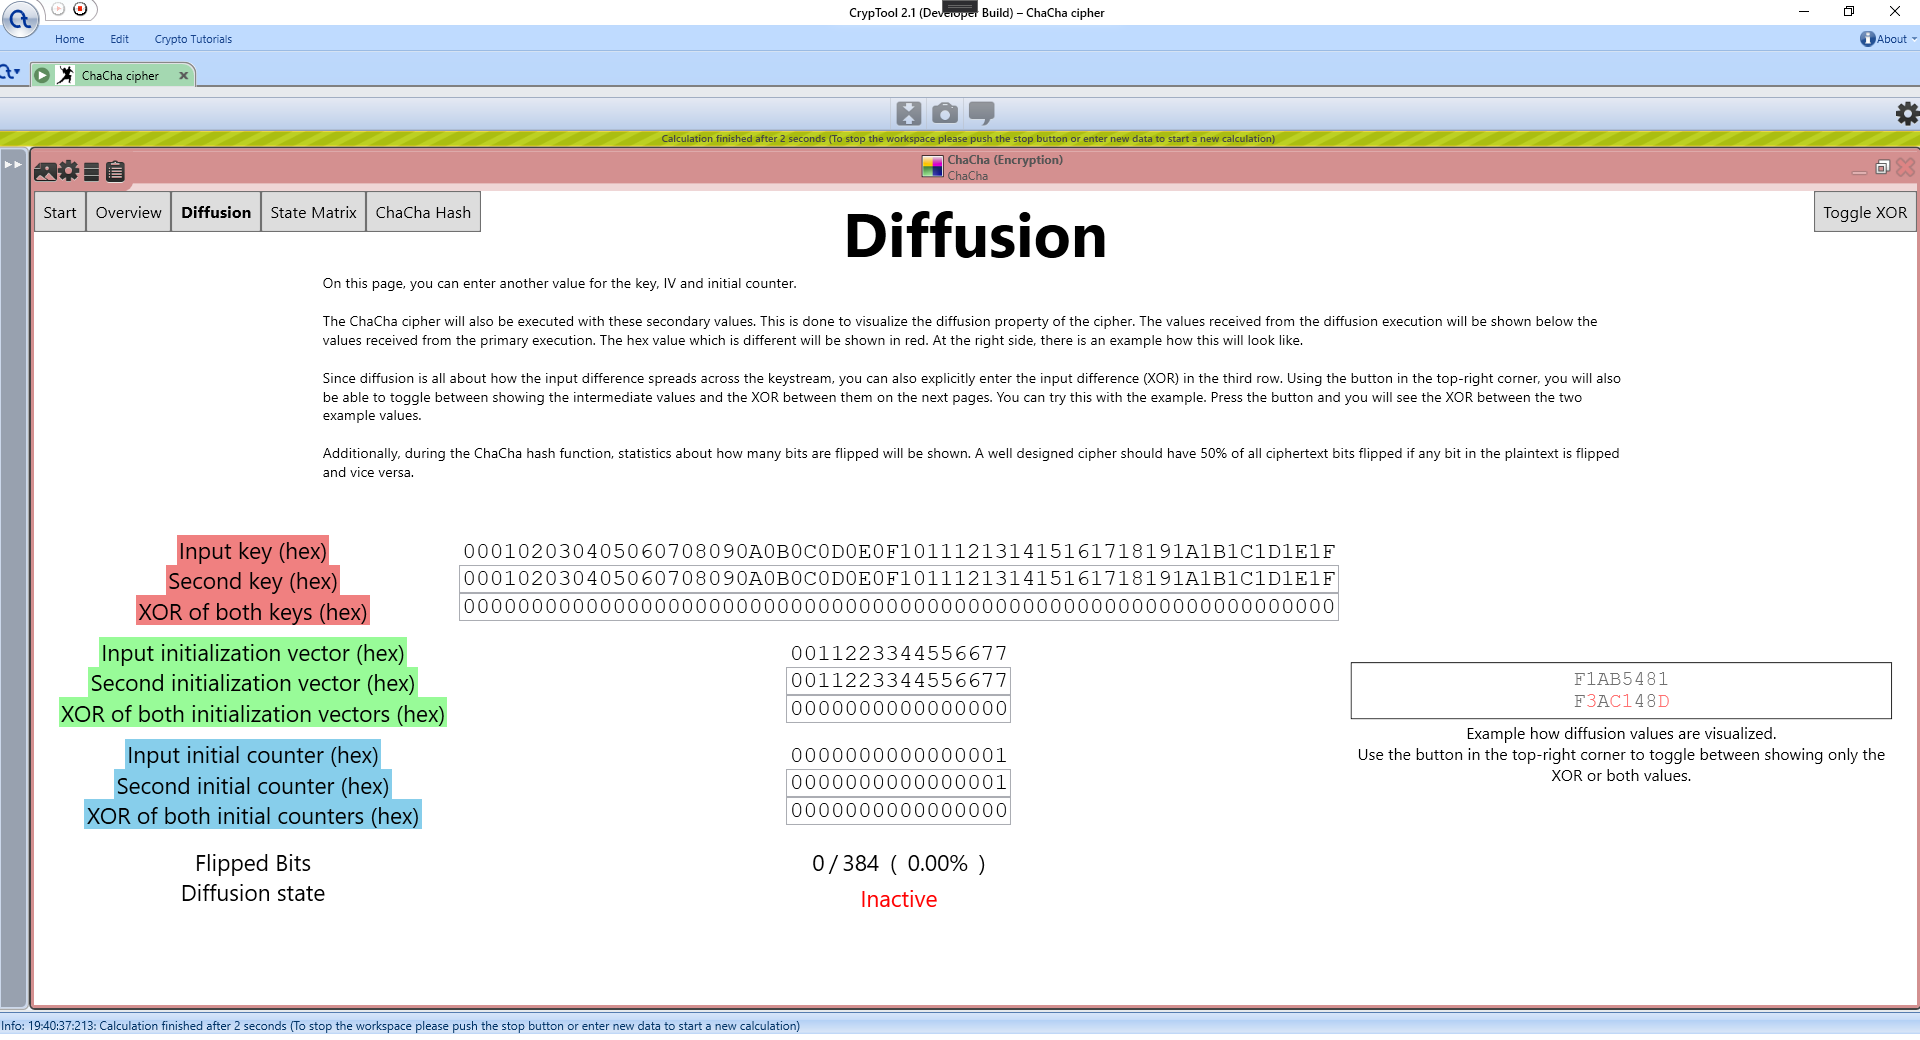
\includegraphics[width=\textwidth]{figures/ct2/all-pages/3-diffusion.png}
  \caption{Diffusion page}
  \label{fig:all-pages.diffusion.page}
\end{subfigure}
\end{figure}
\begin{figure}
\centering
\ContinuedFloat
\begin{subfigure}{\textwidth}
  \centering
  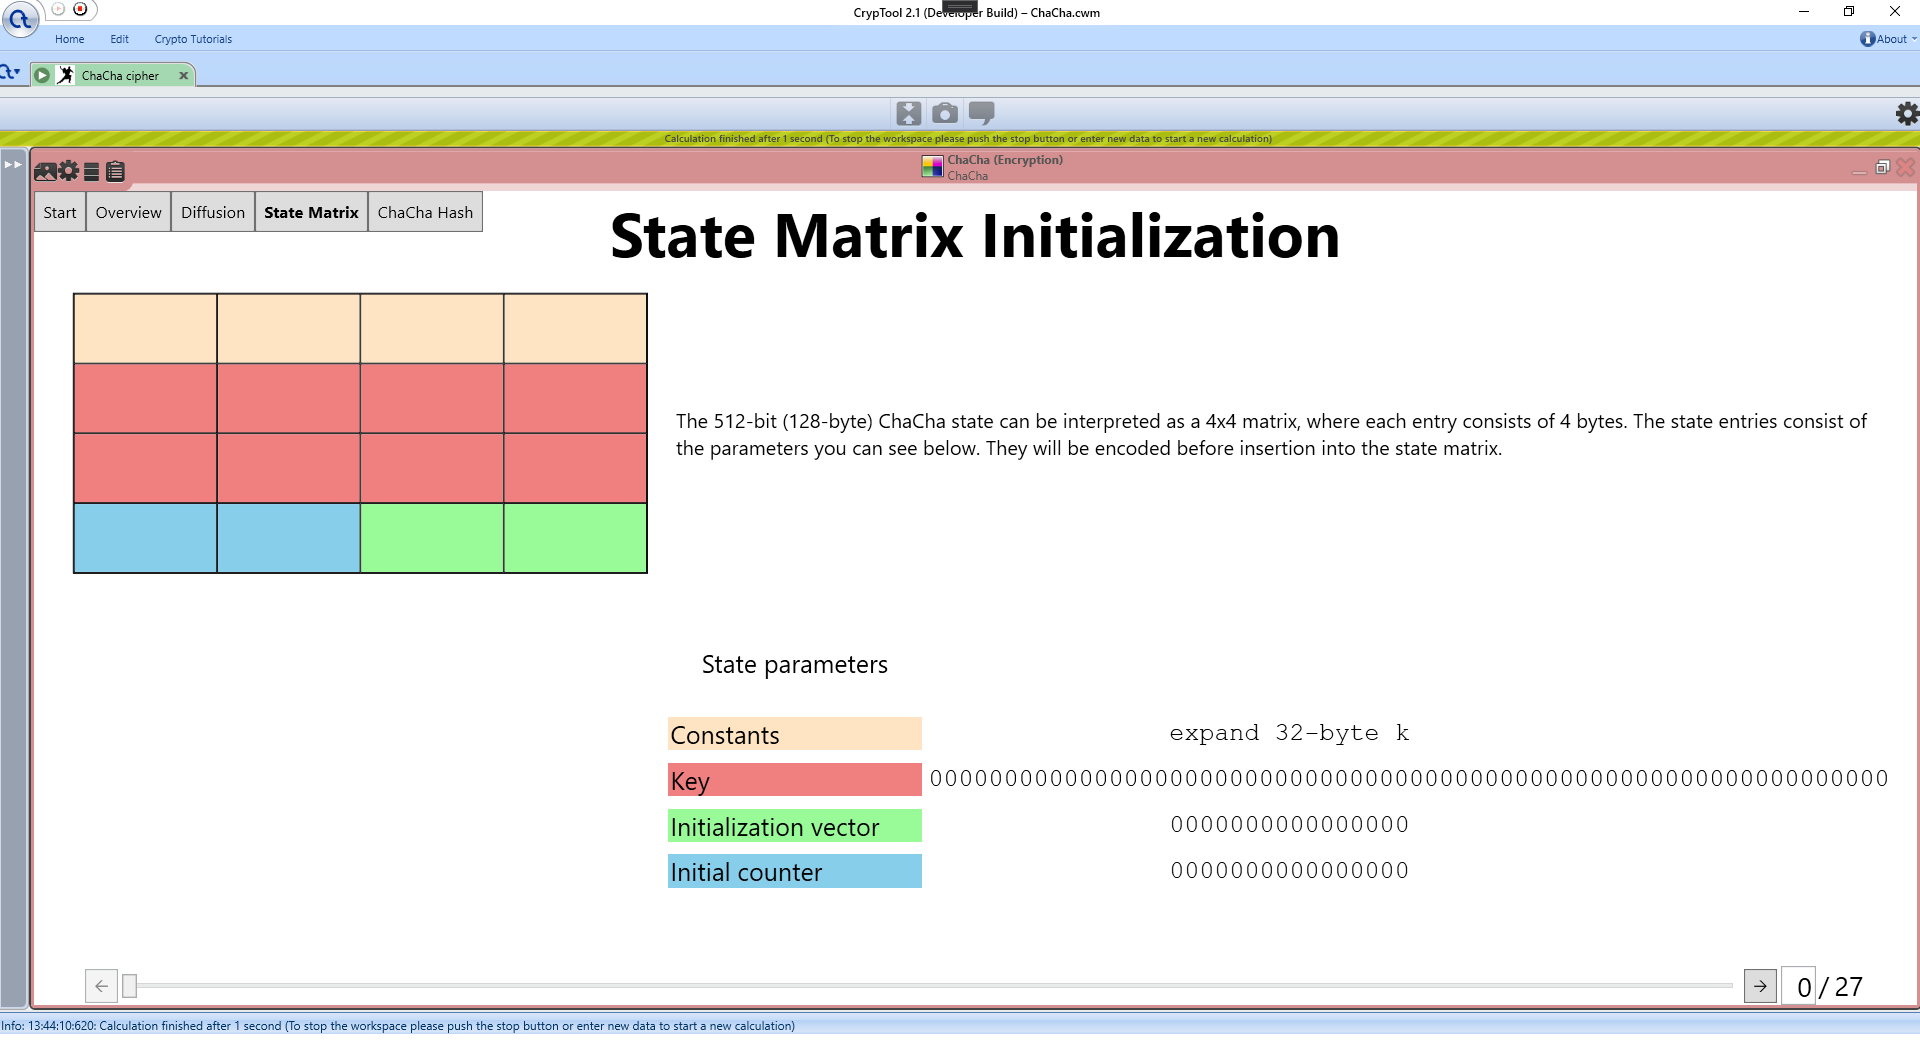
\includegraphics[width=\textwidth]{figures/ct2/all-pages/4-statematrix.png}
  \caption{State Matrix Initialization page}
  \label{fig:all-pages.overview.page}
\end{subfigure}
\begin{subfigure}{\textwidth}
  \centering
  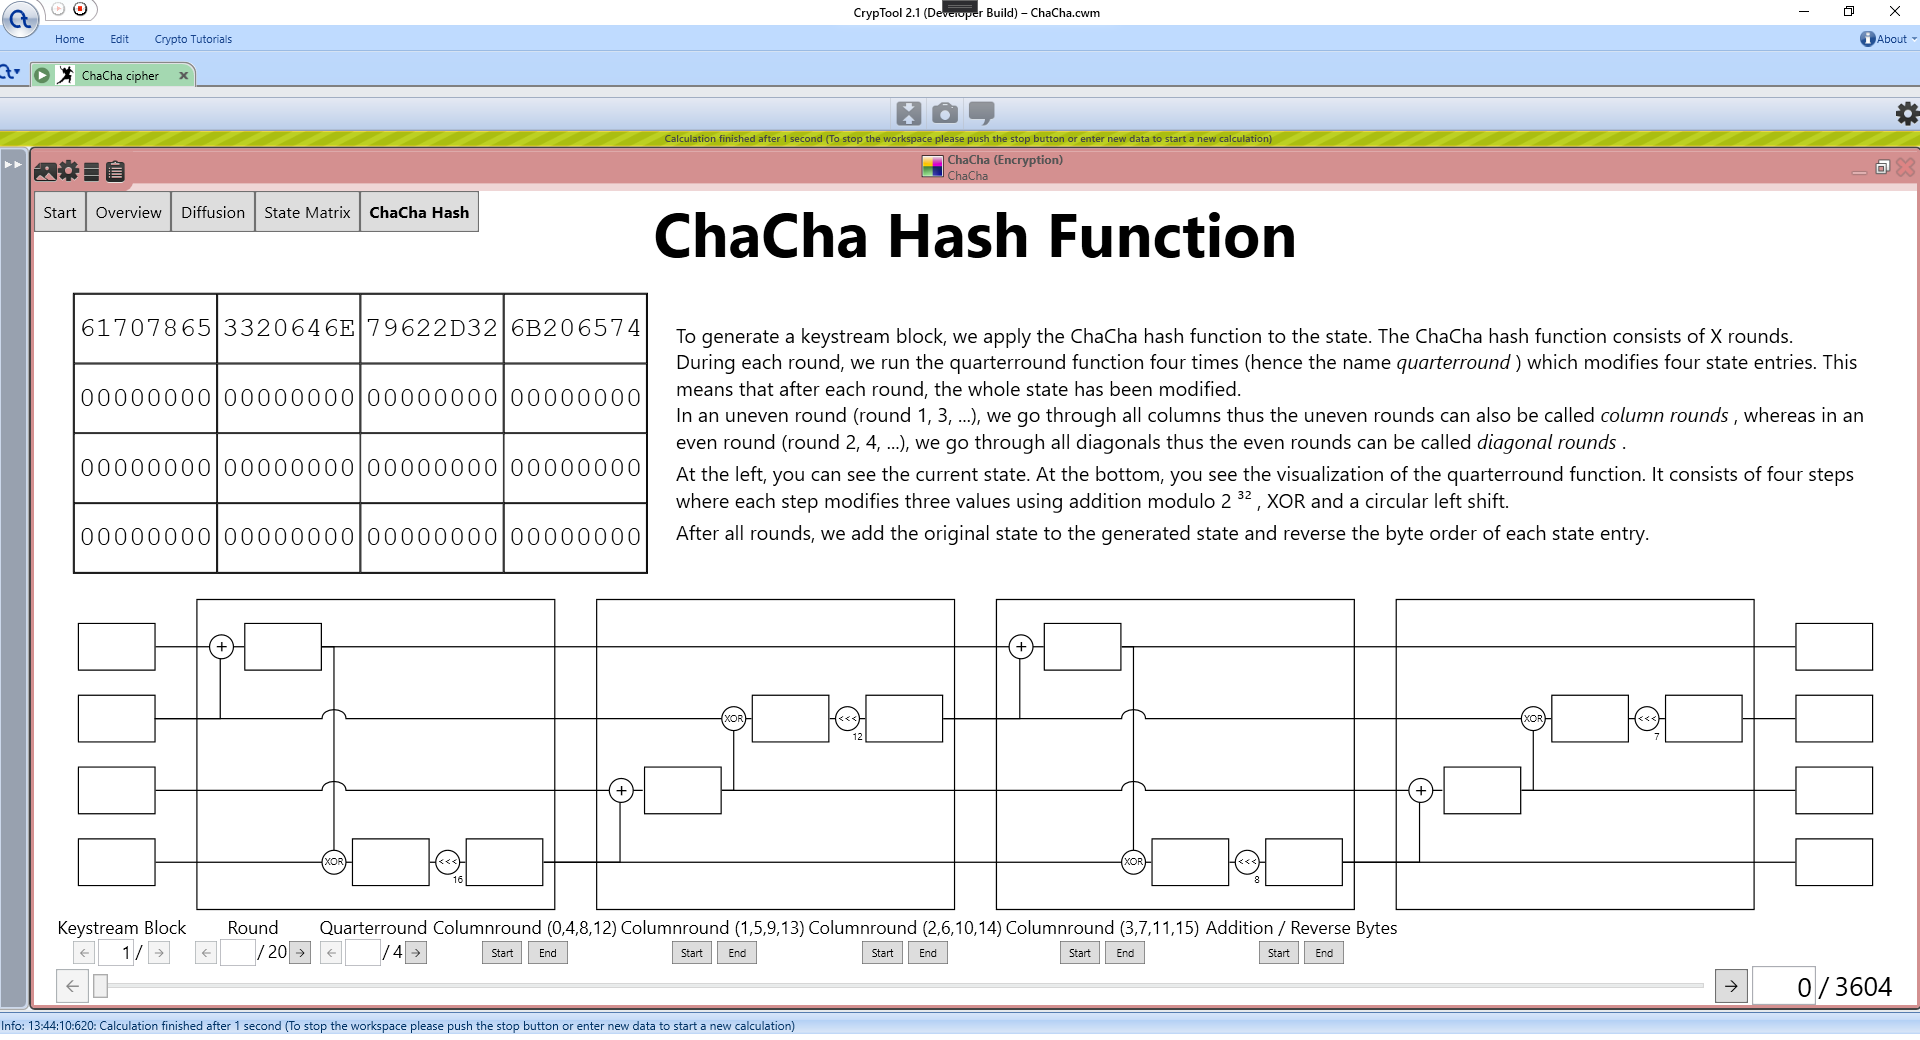
\includegraphics[width=\textwidth]{figures/ct2/all-pages/5-chachahash.png}
  \caption{ChaCha Hash Function page}
  \label{fig:all-pages.chachahash.page}
\end{subfigure}
\caption{All pages of the plug-in in their initial state}
\label{fig:all-pages}
\end{figure}
    
     The visualization is split into five pages in the following order:
     \begin{itemize}
     \item Landing page
     \item Overview page
     \item Diffusion page
     \item State Matrix Initialization page
     \item ChaCha Hash Function page
     \end{itemize}
     Splitting the visualization up into five different pieces (Figure \ref{fig:all-pages}) made it easier to let the user focus on a single step of the encryption process. This also made it possible to have a new page layout for each step without confusing the user because each page is presented as an individual piece. A new page layout for each step was useful because we then were not restricted to a single layout for the whole visualization. Presenting the pages as individual pieces starts with the clear cut from the landing page to the overview page using the page navigation bar in the top-left of each page. 
     
     At the landing page, only the page navigation bar at the top-left is shown. This means the user must use it to advance. After using it, it is clear to the user that this is the place where he can navigate between pages.
     
     Each page tells the user with descriptions what it is about. If a page has actions, the user has access to a slider with buttons in the bottom with which he can navigate within a page. At the bottom-right, the total number of actions a page has is shown as well as a text input which shows the current action index.
     
     Using that text input makes it possible to skip to a certain action. Since the user will not know which action corresponds to which page state when using the plug-in for the first time, additional buttons are shown above the slider which bring the user immediately to important intermediate steps. Looking at the current action index, the user now knows what he has to type in there to immediately jump to that action again. This indirectly helps to better understand the cipher because it enables students and lecturers to talk about a specific step using the action index number.
     
     The state setup and the hash function were visualized with attention to detail. \\
     During the state setup, each parameter is encoded separately and each encoding step is described. During the hash function, the quarter-round circuit diagram makes it possible to show the intermediate results in an intuitive way by placing them above the circuit lines. Intermediate results were important to let the user comprehend every single step of the keystream block generation. Further, background coloring helps to show which elements are used to calculate the next value or which state entries are currently in use by the quarter-round function.
     
     \item \textbf{Visualization of the diffusion property}\\
     The diffusion property is visualized by letting the user enter alternative values on the Diffusion page. Since the ChaCha keystream is independent of the plaintext, the user can only use alternative values for the key, counter and IV.
     
     It was important to easily be able to flip bits. Thus, the user can not only enter the explicit alternative value but also the difference between the two values (XOR).
     
     An example on the same page informs the user what he can expect for the next pages if he activates diffusion by flipping at least one bit. Using the button in the top-right corner enables the user to choose between two vies: \\
     A view which shows both values (as shown in Figure \ref{fig:chachahash.mid.qr.diffusion.both}) and a view to only show the XOR between both values (as shown in Figure \ref{fig:chachahash.mid.qr.diffusion.xor})\\
     The values are always shown in hexadecimal. If a hexadecimal character is different between both cipher runs, it is marked red for easier visual recognition. The two different views were important because when studying the diffusion property of a cipher, one is more interested in the difference between two keystreams instead of their actual values. On the other hand, having access to the concrete values could also be useful thus both views were implemented instead of just one.
     
     Additionally, the percentage of flipped bits is shown below the state at the end of each quarter-round in the ChaCha hash function page.
     
     \item \textbf{Support for all variants of the cipher family}\\
     The support to choose the amount of rounds and the version (original version by Bernstein or IETF version) was implemented by adding appropriate settings to the plug-in. The inputs are then validated accordingly. This means that if the user has chosen the original version by Bernstein, he must enter a 64-bit counter and a 64-bit IV. If he has chosen the IETF version, he must enter a 32-bit counter and a 96-bit IV. The plug-in will not start with wrong inputs. Instead, it will show an error message with the expected size for the input and its actual size.
     
     The visualization works not much different with a 128-bit or 256-bit key. It is mentioned that if using a 128-bit key is used, it will be concatenated with itself. This is done in the step where the encoded key is put into the state.\\
     To reflect the chosen version, only the the overview page and the state setup are slightly different. The overview page shows the correct parameter sizes and the last row of the state in the overview page and state setup page are partitioned accordingly.
  \end{enumerate}

\subsubsection{Main problems (P) and their solutions (S)}

Two main problems were encountered while developing the plug-in.

\begin{enumerate}[label=(\labelenum{P}{{\arabic*}}), wide, labelwidth=!, labelindent=0pt]
\setlength{\parskip}{0pt}

\item \textbf{Architecture}\\
The first problem was to find out how the architecture behind the user interface should be laid out to not hinder further development. This means that it was not straight-forward to know how all systems (user interface, the cipher implementation, navigation, storage and retrieval of intermediate values) should interact without introducing hard-to-debug bugs in the long run.

\item \textbf{Performance}\\
The second problem was the overall performance of the plug-in. It was caused by the desire to let the user navigate to any step within a page. Letting the user navigate from any step to any step meant that the navigation system must support a lot of possible transitions in a reasonable time.

\end{enumerate}

\begin{enumerate}[label=(\labelenum{S}{{\arabic*}}), wide, labelwidth=!, labelindent=0pt]
\setlength{\parskip}{0pt}

\item \textbf{MVVM design pattern}\\
The first problem was solved by following a design pattern. The MVVM design pattern was chosen because it was the most popular across the WPF community. 

Using a design pattern helped in solving a lot of problems in a very obvious way. Features which previously were implemented with a lot of code smells could now be implemented properly without increasing technical debt. \\
For example, before using a design pattern, the navigation system was spread across the whole code base. With the MVVM design pattern, the whole navigation system could be written as a single interface. A abstract view model class then implemented this interface. All other view models which had actions then just extended this base class without having to duplicate any navigational logic.

As mentioned in Section \ref{sec:Architecture}, extensive usage of data binding helped in decoupling the view code from the underlying architecture. Therefore, if some things in the view should change, almost no code in the architecture has to change if the MVVM design pattern is properly implemented. Previously, the view code was very rigid. Changing it took a lot of effort because it kept breaking the architecture behind it.

\item \textbf{Centralized navigation system}\\
The second problem was solved by reflecting on the performance problems previous navigation system implementations had and their underlying issues.

The problem of the first navigation system was that it was designed to execute the transitions in a linear manner (hence the name \textit{linear navigation system}). This meant that skipping a lot of actions would take a lot more time than skipping only a few actions because a lot more transitions needed to be executed for the larger skip. This resulted in taking more than 40 seconds to skip about 3000 actions on the ChaCha hash function page.

This was tried to solve by introducing caches. Even though the cache implementation brought the response time down to 200ms, it did not solve the problem to a satisfactory degree. It introduced inconsistencies regarding the performance because with it, it was not obvious to the user why some skips took longer than others. Before, one could easily see that larger skips took longer than smaller.

As described in Section \ref{sec:Architecture}, as a result, the navigation system was optimized to have a consistently good performance for any skip. This means that the overhead of the navigation system design should be approximately equal for any skip. This was possible with the centralized navigation system. Any transition would start with first going back to the first action and then from there straight to the destination action. Therefore, the start action does not matter because moving to the first action from any action is done in $O(1)$ and moving from the first action to any action is done in $O(1)$. This improved performance dramatically. The average response time was now 5 ms with a maximum response time of about 10 ms.


\end{enumerate}

\section{Future Work}
\label{sec:futureWork}

This section lists suggestions how the plug-in could be further improved to make it more useful for the audience of CrypTool 2.

\begin{enumerate}[wide, labelwidth=!, labelindent=0pt]
\setlength{\parskip}{0pt}

\item \textbf{Better overview over flipped bits at the end of each round}\\
At the end of the Avalanche visualization, the author provided an overview over the percentage of flipped bits at the end of each round. This overview is very useful because it shows how the amount of flipped bits goes up very fast to around 50\% and then stays near it which is exactly what one would expect from a good cipher.

Using a plot instead of the simple text which is updated at the end of each round was considered but due to canvas and time constraints, this idea was not further pursued. 

Nonetheless, integrating such an overview into the Diffusion page should be possible. This would need cipher execution while still on the page instead on page exit but this would not be a big problem since a button to start cipher execution would suffice. Therefore, this plot could be an addition instead of replacing the text below the state in the ChaCha hash function visualization.

\item \textbf{Improve performance during diffusion}\\
All measurements in Section \ref{sec:Architecture} were done with inactive diffusion since the performance during active diffusion improved in a similar manner. This means that thanks to the centralized navigation system architecture, moving to any action is still done in constant time even if diffusion is active.

The problem is that it takes around one or two seconds for each move (instead of around 5 ms if diffusion was inactive) which is quite annoying. We suspect that this is the case because the red color is implemented by creating an inline element for every character and marking it red if it is different.

An idea is to create a single element for every possible combination of color (black and red) and hexadecimal character ([0-9A-F]). Therefore, we would not need to create a new inline element for each character but could reuse the same in multiple places. If the performance issue results from the memory allocation, this approach should solve it. 

However, first attempts resulted in weird bugs. So fixing this will probably be the most difficult point in this list and could result in once again having to rethink some major design decisions.

\item \textbf{Automatic navigation}\\
The AES visualization includes a button labeled with ``Auto''. It lets the visualization run without further user interaction needed. A slider was provided to adjust the speed (see Figure \ref{fig:aes}). 

Such a button could be useful for the ChaCha visualization, too, especially for the page about the ChaCha hash function with its many actions.\\
Since asynchronous navigation is already in use for the action slider, implementing this feature could easily be integrated within the existing navigation system. Only page switches could maybe need some clever solutions since the action navigation is handled within each page thus navigating out of a page may not be straight-forward. 

In the AES visualization though, the automatic navigation does stop between each step (which roughly corresponds to a page in our visualization) so switching the page automatically may even not be desired.

\item \textbf{Salsa20 visualization}\\
As mentioned in Section \ref{sec:salsaCT2Plugin}, using the now existing codebase for ChaCha visualization to create a Salsa20 visualization would definitely increase the value gained from this thesis.

This would at least need adaption of the XAML code for the state matrix initialization and the quarter-round since ChaCha and Salsa20 differ in these aspects from each other. It would most likely even increase the value of the ChaCha visualization since both ciphers could then be compared side-by-side. Comparing them and their diffusion property should be very easy due to the very similar visualization.

\item \textbf{Localization and online help}\\
Currently, most texts are only localized in English. Only the memo fields, component labels and plaintext value are also available in German.\\
This will be changed in the near future. Then also an online help entry for the ChaCha plug-in will be available. The online help appears when pressing F1.

\end{enumerate}

%%%%%%%%%%%%%%%%%%%%%%%%%%%%%%%%%%%%%%%%%%%%%%%%%%%%%%%%%%%%%%%%%%%%%%%%